% Options for packages loaded elsewhere
\PassOptionsToPackage{unicode}{hyperref}
\PassOptionsToPackage{hyphens}{url}
%
\documentclass[
]{article}
\usepackage{amsmath,amssymb}
\usepackage{lmodern}
\usepackage{iftex}
\ifPDFTeX
  \usepackage[T1]{fontenc}
  \usepackage[utf8]{inputenc}
  \usepackage{textcomp} % provide euro and other symbols
\else % if luatex or xetex
  \usepackage{unicode-math}
  \defaultfontfeatures{Scale=MatchLowercase}
  \defaultfontfeatures[\rmfamily]{Ligatures=TeX,Scale=1}
\fi
% Use upquote if available, for straight quotes in verbatim environments
\IfFileExists{upquote.sty}{\usepackage{upquote}}{}
\IfFileExists{microtype.sty}{% use microtype if available
  \usepackage[]{microtype}
  \UseMicrotypeSet[protrusion]{basicmath} % disable protrusion for tt fonts
}{}
\makeatletter
\@ifundefined{KOMAClassName}{% if non-KOMA class
  \IfFileExists{parskip.sty}{%
    \usepackage{parskip}
  }{% else
    \setlength{\parindent}{0pt}
    \setlength{\parskip}{6pt plus 2pt minus 1pt}}
}{% if KOMA class
  \KOMAoptions{parskip=half}}
\makeatother
\usepackage{xcolor}
\usepackage[margin=2.54cm]{geometry}
\usepackage{color}
\usepackage{fancyvrb}
\newcommand{\VerbBar}{|}
\newcommand{\VERB}{\Verb[commandchars=\\\{\}]}
\DefineVerbatimEnvironment{Highlighting}{Verbatim}{commandchars=\\\{\}}
% Add ',fontsize=\small' for more characters per line
\usepackage{framed}
\definecolor{shadecolor}{RGB}{248,248,248}
\newenvironment{Shaded}{\begin{snugshade}}{\end{snugshade}}
\newcommand{\AlertTok}[1]{\textcolor[rgb]{0.94,0.16,0.16}{#1}}
\newcommand{\AnnotationTok}[1]{\textcolor[rgb]{0.56,0.35,0.01}{\textbf{\textit{#1}}}}
\newcommand{\AttributeTok}[1]{\textcolor[rgb]{0.77,0.63,0.00}{#1}}
\newcommand{\BaseNTok}[1]{\textcolor[rgb]{0.00,0.00,0.81}{#1}}
\newcommand{\BuiltInTok}[1]{#1}
\newcommand{\CharTok}[1]{\textcolor[rgb]{0.31,0.60,0.02}{#1}}
\newcommand{\CommentTok}[1]{\textcolor[rgb]{0.56,0.35,0.01}{\textit{#1}}}
\newcommand{\CommentVarTok}[1]{\textcolor[rgb]{0.56,0.35,0.01}{\textbf{\textit{#1}}}}
\newcommand{\ConstantTok}[1]{\textcolor[rgb]{0.00,0.00,0.00}{#1}}
\newcommand{\ControlFlowTok}[1]{\textcolor[rgb]{0.13,0.29,0.53}{\textbf{#1}}}
\newcommand{\DataTypeTok}[1]{\textcolor[rgb]{0.13,0.29,0.53}{#1}}
\newcommand{\DecValTok}[1]{\textcolor[rgb]{0.00,0.00,0.81}{#1}}
\newcommand{\DocumentationTok}[1]{\textcolor[rgb]{0.56,0.35,0.01}{\textbf{\textit{#1}}}}
\newcommand{\ErrorTok}[1]{\textcolor[rgb]{0.64,0.00,0.00}{\textbf{#1}}}
\newcommand{\ExtensionTok}[1]{#1}
\newcommand{\FloatTok}[1]{\textcolor[rgb]{0.00,0.00,0.81}{#1}}
\newcommand{\FunctionTok}[1]{\textcolor[rgb]{0.00,0.00,0.00}{#1}}
\newcommand{\ImportTok}[1]{#1}
\newcommand{\InformationTok}[1]{\textcolor[rgb]{0.56,0.35,0.01}{\textbf{\textit{#1}}}}
\newcommand{\KeywordTok}[1]{\textcolor[rgb]{0.13,0.29,0.53}{\textbf{#1}}}
\newcommand{\NormalTok}[1]{#1}
\newcommand{\OperatorTok}[1]{\textcolor[rgb]{0.81,0.36,0.00}{\textbf{#1}}}
\newcommand{\OtherTok}[1]{\textcolor[rgb]{0.56,0.35,0.01}{#1}}
\newcommand{\PreprocessorTok}[1]{\textcolor[rgb]{0.56,0.35,0.01}{\textit{#1}}}
\newcommand{\RegionMarkerTok}[1]{#1}
\newcommand{\SpecialCharTok}[1]{\textcolor[rgb]{0.00,0.00,0.00}{#1}}
\newcommand{\SpecialStringTok}[1]{\textcolor[rgb]{0.31,0.60,0.02}{#1}}
\newcommand{\StringTok}[1]{\textcolor[rgb]{0.31,0.60,0.02}{#1}}
\newcommand{\VariableTok}[1]{\textcolor[rgb]{0.00,0.00,0.00}{#1}}
\newcommand{\VerbatimStringTok}[1]{\textcolor[rgb]{0.31,0.60,0.02}{#1}}
\newcommand{\WarningTok}[1]{\textcolor[rgb]{0.56,0.35,0.01}{\textbf{\textit{#1}}}}
\usepackage{graphicx}
\makeatletter
\def\maxwidth{\ifdim\Gin@nat@width>\linewidth\linewidth\else\Gin@nat@width\fi}
\def\maxheight{\ifdim\Gin@nat@height>\textheight\textheight\else\Gin@nat@height\fi}
\makeatother
% Scale images if necessary, so that they will not overflow the page
% margins by default, and it is still possible to overwrite the defaults
% using explicit options in \includegraphics[width, height, ...]{}
\setkeys{Gin}{width=\maxwidth,height=\maxheight,keepaspectratio}
% Set default figure placement to htbp
\makeatletter
\def\fps@figure{htbp}
\makeatother
\setlength{\emergencystretch}{3em} % prevent overfull lines
\providecommand{\tightlist}{%
  \setlength{\itemsep}{0pt}\setlength{\parskip}{0pt}}
\setcounter{secnumdepth}{-\maxdimen} % remove section numbering
\ifLuaTeX
  \usepackage{selnolig}  % disable illegal ligatures
\fi
\IfFileExists{bookmark.sty}{\usepackage{bookmark}}{\usepackage{hyperref}}
\IfFileExists{xurl.sty}{\usepackage{xurl}}{} % add URL line breaks if available
\urlstyle{same} % disable monospaced font for URLs
\hypersetup{
  pdftitle={ENV 790.30 - Time Series Analysis for Energy Data \textbar{} Spring 2023},
  pdfauthor={Qiuying Liao},
  hidelinks,
  pdfcreator={LaTeX via pandoc}}

\title{ENV 790.30 - Time Series Analysis for Energy Data \textbar{}
Spring 2023}
\usepackage{etoolbox}
\makeatletter
\providecommand{\subtitle}[1]{% add subtitle to \maketitle
  \apptocmd{\@title}{\par {\large #1 \par}}{}{}
}
\makeatother
\subtitle{Assignment 7 - Due date 03/20/23}
\author{Qiuying Liao}
\date{}

\begin{document}
\maketitle

\hypertarget{directions}{%
\subsection{Directions}\label{directions}}

You should open the .rmd file corresponding to this assignment on
RStudio. The file is available on our class repository on Github. And to
do so you will need to fork our repository and link it to your RStudio.

Once you have the file open on your local machine the first thing you
will do is rename the file such that it includes your first and last
name (e.g., ``LuanaLima\_TSA\_A07\_Sp23.Rmd''). Then change ``Student
Name'' on line 4 with your name.

Then you will start working through the assignment by \textbf{creating
code and output} that answer each question. Be sure to use this
assignment document. Your report should contain the answer to each
question and any plots/tables you obtained (when applicable).

When you have completed the assignment, \textbf{Knit} the text and code
into a single PDF file. Submit this pdf using Sakai.

\hypertarget{set-up}{%
\subsection{Set up}\label{set-up}}

\begin{Shaded}
\begin{Highlighting}[]
\CommentTok{\#Load/install required package here}
\FunctionTok{library}\NormalTok{(}\StringTok{"forecast"}\NormalTok{)}
\end{Highlighting}
\end{Shaded}

\begin{verbatim}
## Registered S3 method overwritten by 'quantmod':
##   method            from
##   as.zoo.data.frame zoo
\end{verbatim}

\begin{Shaded}
\begin{Highlighting}[]
\FunctionTok{library}\NormalTok{(}\StringTok{"tseries"}\NormalTok{)}
\FunctionTok{library}\NormalTok{(}\StringTok{"dplyr"}\NormalTok{)}
\end{Highlighting}
\end{Shaded}

\begin{verbatim}
## 
## Attaching package: 'dplyr'
\end{verbatim}

\begin{verbatim}
## The following objects are masked from 'package:stats':
## 
##     filter, lag
\end{verbatim}

\begin{verbatim}
## The following objects are masked from 'package:base':
## 
##     intersect, setdiff, setequal, union
\end{verbatim}

\begin{Shaded}
\begin{Highlighting}[]
\FunctionTok{library}\NormalTok{(}\StringTok{"ggplot2"}\NormalTok{)}
\FunctionTok{library}\NormalTok{(}\StringTok{"Kendall"}\NormalTok{)}
\end{Highlighting}
\end{Shaded}

\hypertarget{importing-and-processing-the-data-set}{%
\subsection{Importing and processing the data
set}\label{importing-and-processing-the-data-set}}

Consider the data from the file
``Net\_generation\_United\_States\_all\_sectors\_monthly.csv''. The data
corresponds to the monthly net generation from January 2001 to December
2020 by source and is provided by the US Energy Information and
Administration. \textbf{You will work with the natural gas column only}.

Packages needed for this assignment: ``forecast'',``tseries''. Do not
forget to load them before running your script, since they are NOT
default packages.\textbackslash{}

\hypertarget{q1}{%
\subsubsection{Q1}\label{q1}}

Import the csv file and create a time series object for natural gas.
Make you sure you specify the \textbf{start=} and \textbf{frequency=}
arguments. Plot the time series over time, ACF and PACF.

\begin{Shaded}
\begin{Highlighting}[]
\CommentTok{\#import data}
\NormalTok{energy\_df }\OtherTok{\textless{}{-}} \FunctionTok{read.csv}\NormalTok{(}\StringTok{"../Data/Net\_generation\_United\_States\_all\_sectors\_monthly.csv"}\NormalTok{, }\AttributeTok{header=}\ConstantTok{TRUE}\NormalTok{, }\AttributeTok{skip=}\DecValTok{4}\NormalTok{)}

\CommentTok{\#Take out Natural gas}
\NormalTok{energy\_df\_NG}\OtherTok{\textless{}{-}}\NormalTok{energy\_df[,}\FunctionTok{c}\NormalTok{(}\StringTok{"Month"}\NormalTok{,}\StringTok{"natural.gas.thousand.megawatthours"}\NormalTok{)]}
\FunctionTok{head}\NormalTok{(energy\_df\_NG)}
\end{Highlighting}
\end{Shaded}

\begin{verbatim}
##      Month natural.gas.thousand.megawatthours
## 1 Dec 2020                           125703.7
## 2 Nov 2020                           109037.2
## 3 Oct 2020                           131658.2
## 4 Sep 2020                           141452.7
## 5 Aug 2020                           173926.6
## 6 Jul 2020                           185444.8
\end{verbatim}

\begin{Shaded}
\begin{Highlighting}[]
\CommentTok{\#rename columns}
\NormalTok{energy\_df\_NG }\OtherTok{\textless{}{-}}\NormalTok{ energy\_df\_NG }\SpecialCharTok{\%\textgreater{}\%}
  \FunctionTok{rename}\NormalTok{(}\StringTok{"Month"} \OtherTok{=} \DecValTok{1}\NormalTok{,}\StringTok{"Natural Gas"} \OtherTok{=} \DecValTok{2}\NormalTok{)}
\FunctionTok{head}\NormalTok{(energy\_df\_NG)}
\end{Highlighting}
\end{Shaded}

\begin{verbatim}
##      Month Natural Gas
## 1 Dec 2020    125703.7
## 2 Nov 2020    109037.2
## 3 Oct 2020    131658.2
## 4 Sep 2020    141452.7
## 5 Aug 2020    173926.6
## 6 Jul 2020    185444.8
\end{verbatim}

\begin{Shaded}
\begin{Highlighting}[]
\CommentTok{\#convert month format}
\NormalTok{Date}\OtherTok{\textless{}{-}}\FunctionTok{paste}\NormalTok{(energy\_df\_NG[,}\DecValTok{1}\NormalTok{],}\StringTok{"01"}\NormalTok{,}\AttributeTok{sep=}\StringTok{""}\NormalTok{)}
\NormalTok{Date\_new}\OtherTok{\textless{}{-}}\FunctionTok{as.Date}\NormalTok{(Date,}\AttributeTok{format=}\StringTok{"\%Y \%B"}\NormalTok{)}
\FunctionTok{head}\NormalTok{(Date\_new)}
\end{Highlighting}
\end{Shaded}

\begin{verbatim}
## [1] NA NA NA NA NA NA
\end{verbatim}

\begin{Shaded}
\begin{Highlighting}[]
\CommentTok{\#time series}
\NormalTok{ts\_energy\_df\_NG }\OtherTok{\textless{}{-}} \FunctionTok{ts}\NormalTok{(energy\_df\_NG[,}\DecValTok{2}\NormalTok{], }\AttributeTok{start =} \FunctionTok{c}\NormalTok{(}\DecValTok{2001}\NormalTok{,}\DecValTok{1}\NormalTok{), }\AttributeTok{frequency =} \DecValTok{12}\NormalTok{)}
\end{Highlighting}
\end{Shaded}

\begin{Shaded}
\begin{Highlighting}[]
\CommentTok{\#acf and pacf of the time series}
\FunctionTok{par}\NormalTok{(}\AttributeTok{mfrow=}\FunctionTok{c}\NormalTok{(}\DecValTok{1}\NormalTok{,}\DecValTok{3}\NormalTok{))}
\FunctionTok{plot}\NormalTok{(ts\_energy\_df\_NG, }\AttributeTok{xlab=}\StringTok{"Time"}\NormalTok{, }\AttributeTok{ylab=}\StringTok{"Natural Gas (thousand MWh)"}\NormalTok{, }\AttributeTok{main =} \StringTok{"Time Series of Natural Gas"}\NormalTok{)}
\FunctionTok{acf}\NormalTok{(ts\_energy\_df\_NG, }\AttributeTok{lag=}\DecValTok{40}\NormalTok{, }\AttributeTok{main =} \StringTok{"ACF of Natural Gas"}\NormalTok{)}
\FunctionTok{pacf}\NormalTok{(ts\_energy\_df\_NG, }\AttributeTok{lag=}\DecValTok{40}\NormalTok{, }\AttributeTok{main =} \StringTok{"PACF of Natural Gas "}\NormalTok{)}
\end{Highlighting}
\end{Shaded}

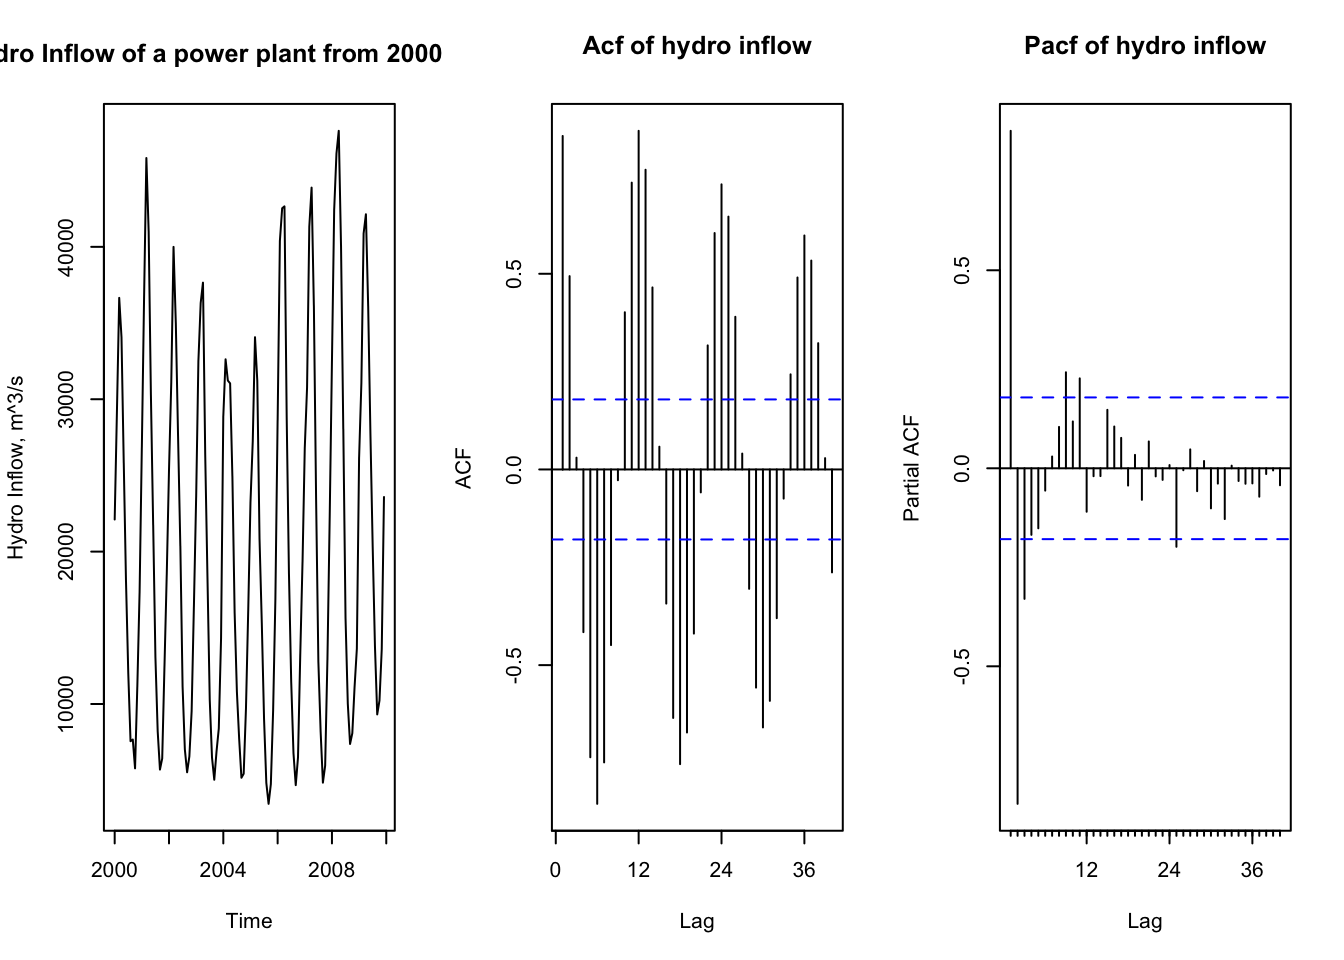
\includegraphics{QiuyingLiao_TSA_A7_Mar20_files/figure-latex/unnamed-chunk-3-1.pdf}

\hypertarget{q2}{%
\subsubsection{Q2}\label{q2}}

Using the \(decompose()\) or \(stl()\) and the \(seasadj()\) functions
create a series without the seasonal component, i.e., a deseasonalized
natural gas series. Plot the deseasonalized series over time and
corresponding ACF and PACF. Compare with the plots obtained in Q1.

\begin{Shaded}
\begin{Highlighting}[]
\CommentTok{\#decompose}
\NormalTok{decompose\_NG }\OtherTok{\textless{}{-}} \FunctionTok{decompose}\NormalTok{(ts\_energy\_df\_NG, }\StringTok{"additive"}\NormalTok{) }
\FunctionTok{plot}\NormalTok{(decompose\_NG)}
\end{Highlighting}
\end{Shaded}

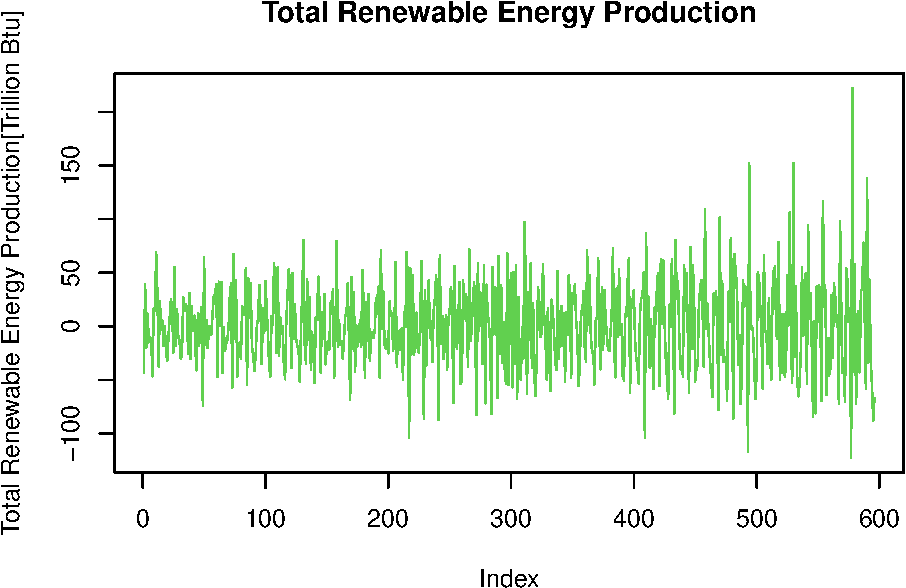
\includegraphics{QiuyingLiao_TSA_A7_Mar20_files/figure-latex/unnamed-chunk-4-1.pdf}

\begin{Shaded}
\begin{Highlighting}[]
\CommentTok{\#create non{-}seasonal natural gas time series}
\CommentTok{\#seasonal adjustment to original data, only works for decompose}
\NormalTok{deseasonal\_NG }\OtherTok{\textless{}{-}} \FunctionTok{seasadj}\NormalTok{(decompose\_NG) }
\FunctionTok{plot}\NormalTok{(deseasonal\_NG)}
\end{Highlighting}
\end{Shaded}

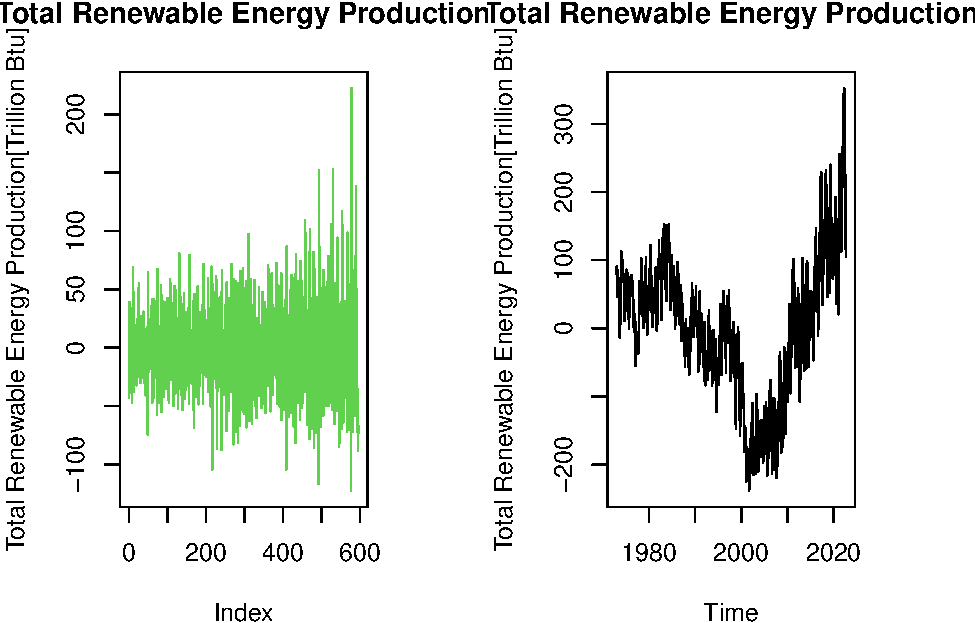
\includegraphics{QiuyingLiao_TSA_A7_Mar20_files/figure-latex/unnamed-chunk-5-1.pdf}

\begin{Shaded}
\begin{Highlighting}[]
\CommentTok{\#Comparing ACFs}
\CommentTok{\#seasonality is removed}
\FunctionTok{par}\NormalTok{(}\AttributeTok{mar=}\FunctionTok{c}\NormalTok{(}\DecValTok{3}\NormalTok{,}\DecValTok{3}\NormalTok{,}\DecValTok{3}\NormalTok{,}\DecValTok{0}\NormalTok{));}\FunctionTok{par}\NormalTok{(}\AttributeTok{mfrow=}\FunctionTok{c}\NormalTok{(}\DecValTok{1}\NormalTok{,}\DecValTok{2}\NormalTok{))}
\FunctionTok{Acf}\NormalTok{(deseasonal\_NG,}\AttributeTok{lag.max=}\DecValTok{40}\NormalTok{,}\AttributeTok{main=}\StringTok{"ACF of Non Sesonal Natural Gas"}\NormalTok{)}
\FunctionTok{Pacf}\NormalTok{(deseasonal\_NG,}\AttributeTok{lag.max=}\DecValTok{40}\NormalTok{,}\AttributeTok{main=}\StringTok{"PACF of Non Sesonal Natural Gas"}\NormalTok{)}
\end{Highlighting}
\end{Shaded}

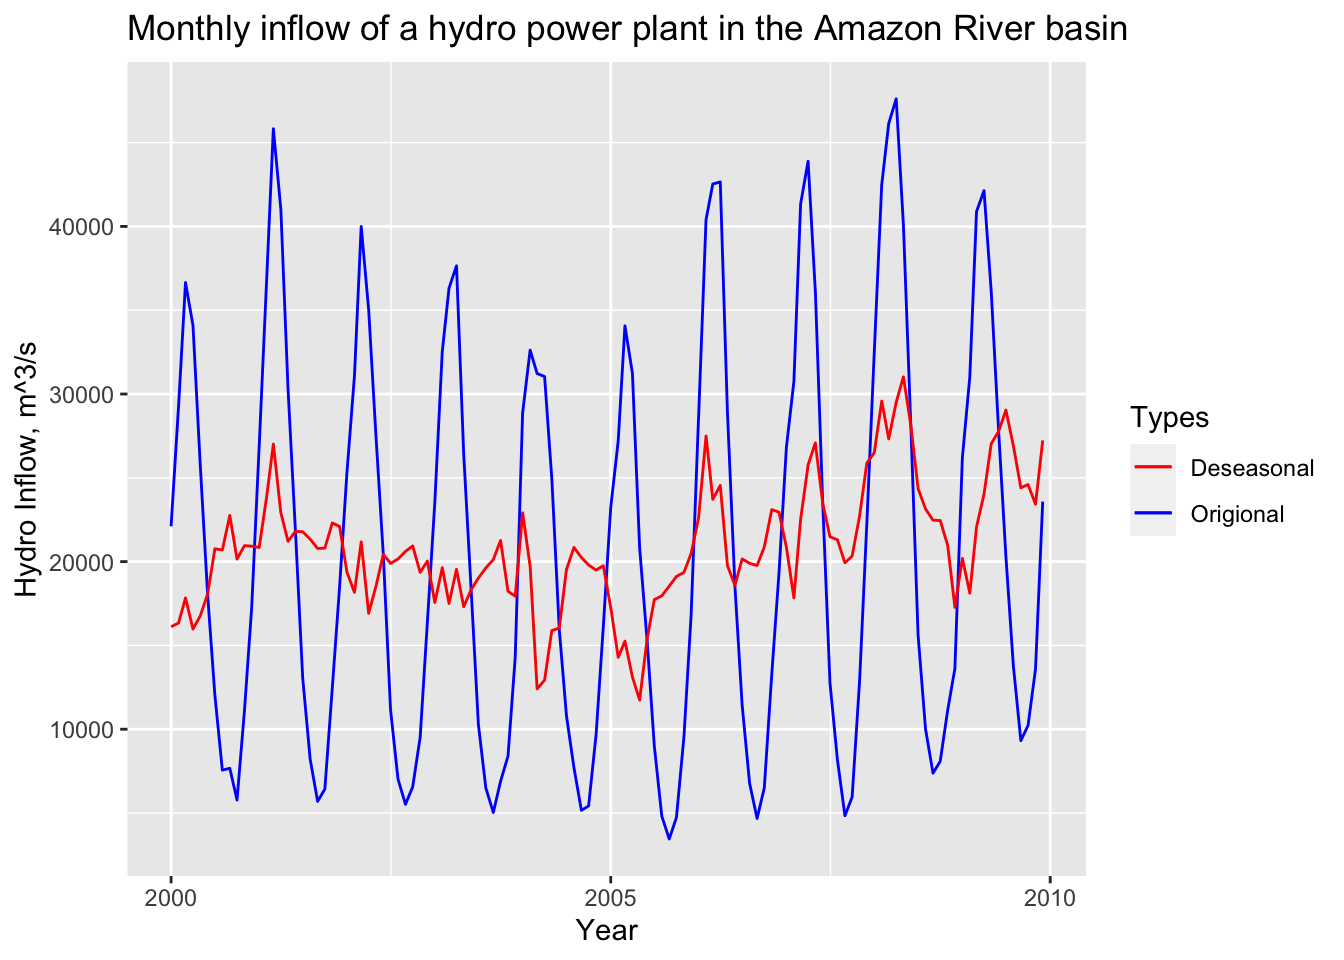
\includegraphics{QiuyingLiao_TSA_A7_Mar20_files/figure-latex/unnamed-chunk-6-1.pdf}

\begin{quote}
Answer: Compared with the plots obtained in Q1, the acf of nonseasonal
natural gas have slow decay instead of seasonal spike. Therefore, we
removed the seasonality. Also, we removed those little spikes for the
seasonality in the pacf of nonseasonal natural gas compared to the pacf
of natural gas.
\end{quote}

\hypertarget{modeling-the-seasonally-adjusted-or-deseasonalized-series}{%
\subsection{Modeling the seasonally adjusted or deseasonalized
series}\label{modeling-the-seasonally-adjusted-or-deseasonalized-series}}

\hypertarget{q3}{%
\subsubsection{Q3}\label{q3}}

Run the ADF test and Mann Kendall test on the deseasonalized data from
Q2. Report and explain the results.

\begin{Shaded}
\begin{Highlighting}[]
\CommentTok{\#Run ADF, check for stationarity}
\CommentTok{\#adf.test(deseasonal\_NG,alternative="stationary")}
\FunctionTok{print}\NormalTok{((}\FunctionTok{adf.test}\NormalTok{(deseasonal\_NG, }\AttributeTok{alternative =}\StringTok{"stationary"}\NormalTok{)))}
\end{Highlighting}
\end{Shaded}

\begin{verbatim}
## Warning in adf.test(deseasonal_NG, alternative = "stationary"): p-value smaller
## than printed p-value
\end{verbatim}

\begin{verbatim}
## 
##  Augmented Dickey-Fuller Test
## 
## data:  deseasonal_NG
## Dickey-Fuller = -4.0574, Lag order = 6, p-value = 0.01
## alternative hypothesis: stationary
\end{verbatim}

\begin{Shaded}
\begin{Highlighting}[]
\CommentTok{\#Run Mann Kendall test to check for stationarity}
\NormalTok{MKtest }\OtherTok{\textless{}{-}} \FunctionTok{MannKendall}\NormalTok{(deseasonal\_NG)}
\FunctionTok{print}\NormalTok{(}\StringTok{"Results for Mann Kendall /n"}\NormalTok{)}
\end{Highlighting}
\end{Shaded}

\begin{verbatim}
## [1] "Results for Mann Kendall /n"
\end{verbatim}

\begin{Shaded}
\begin{Highlighting}[]
\FunctionTok{print}\NormalTok{(}\FunctionTok{summary}\NormalTok{(MKtest))}
\end{Highlighting}
\end{Shaded}

\begin{verbatim}
## Score =  -24186 , Var(Score) = 1545533
## denominator =  28680
## tau = -0.843, 2-sided pvalue =< 2.22e-16
## NULL
\end{verbatim}

\begin{quote}
Answer:The p-value for ADF is 0.01, which is smaller than 0.05 and we
can reject the null hypothesis. Therefore, we can say that the
stochastic trend is stationary. The p-value for MannKendall test is
smaller than 0.05, and we can reject the null hypothesis. Therefore, we
can say that there is a deterministic trend. We need to difference it to
remove the trend, so d=1.
\end{quote}

\hypertarget{q4}{%
\subsubsection{Q4}\label{q4}}

Using the plots from Q2 and test results from Q3 identify the ARIMA
model parameters \(p,d\) and \(q\). Note that in this case because you
removed the seasonal component prior to identifying the model you don't
need to worry about seasonal component. Clearly state your criteria and
any additional function in R you might use. DO NOT use the
\(auto.arima()\) function. You will be evaluated on ability to can read
the plots and interpret the test results.

\begin{Shaded}
\begin{Highlighting}[]
\CommentTok{\# Find out how many time we need to difference}
\NormalTok{n\_diff }\OtherTok{\textless{}{-}} \FunctionTok{ndiffs}\NormalTok{(deseasonal\_NG)}
\FunctionTok{cat}\NormalTok{(}\StringTok{"Number of differencing needed: "}\NormalTok{,n\_diff) }
\end{Highlighting}
\end{Shaded}

\begin{verbatim}
## Number of differencing needed:  1
\end{verbatim}

\begin{quote}
Answer: p=2, because there are 2 spike that are above the significant
level from PACF graph, which is the cutoff; q=0, because the ACF of the
graph tails off and has slow decays; d=1, we got this value from the
ndiffs. (p,d,q) = (2,1,0)
\end{quote}

\hypertarget{q5}{%
\subsubsection{Q5}\label{q5}}

Use \(Arima()\) from package ``forecast'' to fit an ARIMA model to your
series considering the order estimated in Q4. You should allow constants
in the model, i.e., \(include.mean = TRUE\) or \(include.drift=TRUE\).
\textbf{Print the coefficients} in your report. Hint: use the \(cat()\)
function to print.

\begin{Shaded}
\begin{Highlighting}[]
\CommentTok{\#Now let\textquotesingle{}s try ARIMA(2,1,0)}
\NormalTok{Model\_210 }\OtherTok{\textless{}{-}} \FunctionTok{Arima}\NormalTok{(deseasonal\_NG,}\AttributeTok{order=}\FunctionTok{c}\NormalTok{(}\DecValTok{2}\NormalTok{,}\DecValTok{1}\NormalTok{,}\DecValTok{0}\NormalTok{),}\AttributeTok{include.drift=}\ConstantTok{TRUE}\NormalTok{)}
\FunctionTok{print}\NormalTok{(Model\_210)}
\end{Highlighting}
\end{Shaded}

\begin{verbatim}
## Series: deseasonal_NG 
## ARIMA(2,1,0) with drift 
## 
## Coefficients:
##           ar1      ar2      drift
##       -0.1647  -0.1283  -346.9085
## s.e.   0.0645   0.0650   272.1652
## 
## sigma^2 = 29891484:  log likelihood = -2394.61
## AIC=4797.21   AICc=4797.39   BIC=4811.12
\end{verbatim}

\begin{Shaded}
\begin{Highlighting}[]
\FunctionTok{cat}\NormalTok{(}\StringTok{"Coefficient is"}\NormalTok{,Model\_210}\SpecialCharTok{$}\NormalTok{coef)}
\end{Highlighting}
\end{Shaded}

\begin{verbatim}
## Coefficient is -0.1647187 -0.1283153 -346.9085
\end{verbatim}

\hypertarget{q6}{%
\subsubsection{Q6}\label{q6}}

Now plot the residuals of the ARIMA fit from Q5 along with residuals ACF
and PACF on the same window. You may use the \(checkresiduals()\)
function to automatically generate the three plots. Do the residual
series look like a white noise series? Why?

\begin{quote}
Answer: the residual series look like a white noise series because
variables are independent and identically distributed with a mean of
zero.
\end{quote}

\begin{Shaded}
\begin{Highlighting}[]
\FunctionTok{checkresiduals}\NormalTok{(Model\_210)}
\end{Highlighting}
\end{Shaded}

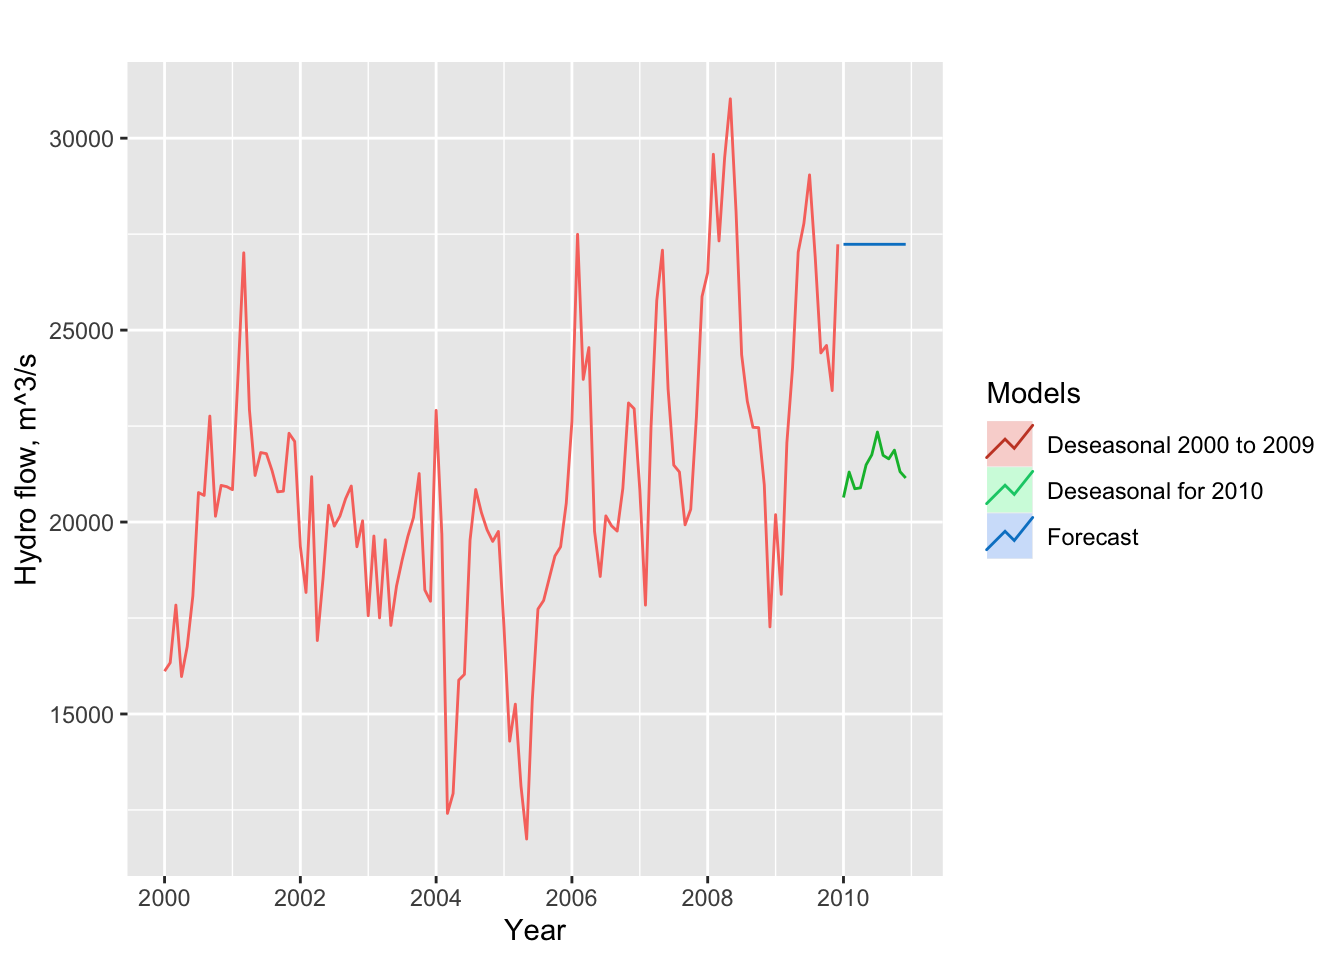
\includegraphics{QiuyingLiao_TSA_A7_Mar20_files/figure-latex/unnamed-chunk-10-1.pdf}

\begin{verbatim}
## 
##  Ljung-Box test
## 
## data:  Residuals from ARIMA(2,1,0) with drift
## Q* = 74.829, df = 22, p-value = 1.126e-07
## 
## Model df: 2.   Total lags used: 24
\end{verbatim}

\begin{Shaded}
\begin{Highlighting}[]
\CommentTok{\#Check residuals series, if white noise we got a good fit}
\FunctionTok{par}\NormalTok{(}\AttributeTok{mar=}\FunctionTok{c}\NormalTok{(}\DecValTok{3}\NormalTok{,}\DecValTok{3}\NormalTok{,}\DecValTok{3}\NormalTok{,}\DecValTok{0}\NormalTok{));}\FunctionTok{par}\NormalTok{(}\AttributeTok{mfrow=}\FunctionTok{c}\NormalTok{(}\DecValTok{1}\NormalTok{,}\DecValTok{3}\NormalTok{))}
\FunctionTok{ts.plot}\NormalTok{(Model\_210}\SpecialCharTok{$}\NormalTok{residuals)}
\FunctionTok{Acf}\NormalTok{(Model\_210}\SpecialCharTok{$}\NormalTok{residuals,}\AttributeTok{lag.max=}\DecValTok{40}\NormalTok{)}
\FunctionTok{Pacf}\NormalTok{(Model\_210}\SpecialCharTok{$}\NormalTok{residuals,}\AttributeTok{lag.max=}\DecValTok{40}\NormalTok{)}
\end{Highlighting}
\end{Shaded}

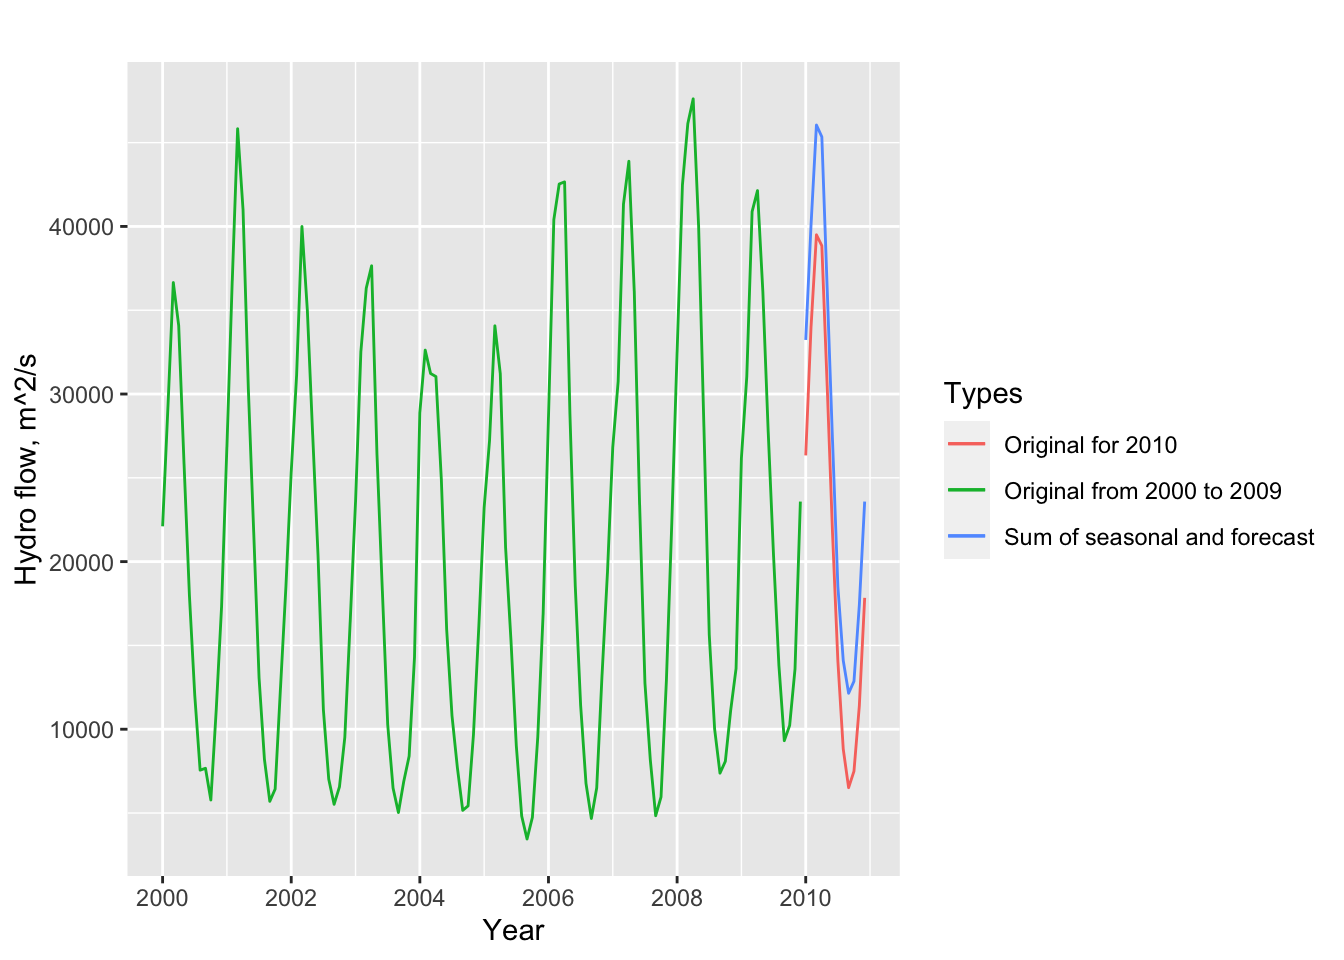
\includegraphics{QiuyingLiao_TSA_A7_Mar20_files/figure-latex/unnamed-chunk-11-1.pdf}

\hypertarget{modeling-the-original-series-with-seasonality}{%
\subsection{Modeling the original series (with
seasonality)}\label{modeling-the-original-series-with-seasonality}}

\hypertarget{q7}{%
\subsubsection{Q7}\label{q7}}

Repeat Q4-Q6 for the original series (the complete series that has the
seasonal component). Note that when you model the seasonal series, you
need to specify the seasonal part of the ARIMA model as well, i.e.,
\(P\), \(D\) and \(Q\).

\begin{Shaded}
\begin{Highlighting}[]
\CommentTok{\# Find out how many time we need to difference}
\NormalTok{ns\_diff }\OtherTok{\textless{}{-}} \FunctionTok{nsdiffs}\NormalTok{(ts\_energy\_df\_NG)}
\FunctionTok{cat}\NormalTok{(}\StringTok{"Number of seasonal differencing needed: "}\NormalTok{,ns\_diff)}
\end{Highlighting}
\end{Shaded}

\begin{verbatim}
## Number of seasonal differencing needed:  1
\end{verbatim}

\begin{Shaded}
\begin{Highlighting}[]
\CommentTok{\#Lets difference the series once at lag 12 to remove the seasonal trend.}
\NormalTok{NG\_seas\_diff }\OtherTok{\textless{}{-}} \FunctionTok{diff}\NormalTok{(ts\_energy\_df\_NG,}\AttributeTok{lag=}\DecValTok{12}\NormalTok{, }\AttributeTok{differences=}\DecValTok{1}\NormalTok{) }\CommentTok{\#difference at seasonal lag, differncing 1}
\NormalTok{NG\_trend\_diff }\OtherTok{\textless{}{-}} \FunctionTok{diff}\NormalTok{(ts\_energy\_df\_NG,}\AttributeTok{lag =}\DecValTok{1}\NormalTok{, }\AttributeTok{differences=}\DecValTok{1}\NormalTok{) }\CommentTok{\#diff done on orig series}
\NormalTok{NG\_both\_diff }\OtherTok{\textless{}{-}} \FunctionTok{diff}\NormalTok{(NG\_trend\_diff,}\AttributeTok{lag =}\DecValTok{12}\NormalTok{, }\AttributeTok{differences=}\DecValTok{1}\NormalTok{)}
\end{Highlighting}
\end{Shaded}

\begin{Shaded}
\begin{Highlighting}[]
\CommentTok{\#Check autocorrelation plots for differenced series}
\CommentTok{\#Comparing ACFs}
\FunctionTok{par}\NormalTok{(}\AttributeTok{mfrow=}\FunctionTok{c}\NormalTok{(}\DecValTok{1}\NormalTok{,}\DecValTok{4}\NormalTok{))}
\FunctionTok{Acf}\NormalTok{(ts\_energy\_df\_NG,}\AttributeTok{lag.max=}\DecValTok{40}\NormalTok{,}\AttributeTok{main=}\StringTok{"Natural Gas"}\NormalTok{,}\AttributeTok{ylim=}\FunctionTok{c}\NormalTok{(}\SpecialCharTok{{-}}\DecValTok{1}\NormalTok{,}\DecValTok{1}\NormalTok{))}
\FunctionTok{Acf}\NormalTok{(NG\_seas\_diff ,}\AttributeTok{lag.max=}\DecValTok{60}\NormalTok{,}\AttributeTok{main=}\StringTok{"Seasonal{-}Differenced Natural Gas"}\NormalTok{,}\AttributeTok{ylim=}\FunctionTok{c}\NormalTok{(}\SpecialCharTok{{-}}\DecValTok{1}\NormalTok{,}\DecValTok{1}\NormalTok{)) }\CommentTok{\#at lag 12}
\FunctionTok{Acf}\NormalTok{(NG\_trend\_diff,}\AttributeTok{lag.max=}\DecValTok{60}\NormalTok{,}\AttributeTok{main=}\StringTok{"Trend{-}Differenced Natural Gas"}\NormalTok{,}\AttributeTok{ylim=}\FunctionTok{c}\NormalTok{(}\SpecialCharTok{{-}}\DecValTok{1}\NormalTok{,}\DecValTok{1}\NormalTok{)) }\CommentTok{\#at lag 1}
\FunctionTok{Acf}\NormalTok{(NG\_both\_diff,}\AttributeTok{lag.max=}\DecValTok{60}\NormalTok{,}\AttributeTok{main=}\StringTok{"Twice{-}Differenced Natural Gas"}\NormalTok{,}\AttributeTok{ylim=}\FunctionTok{c}\NormalTok{(}\SpecialCharTok{{-}}\DecValTok{1}\NormalTok{,}\DecValTok{1}\NormalTok{))}
\end{Highlighting}
\end{Shaded}

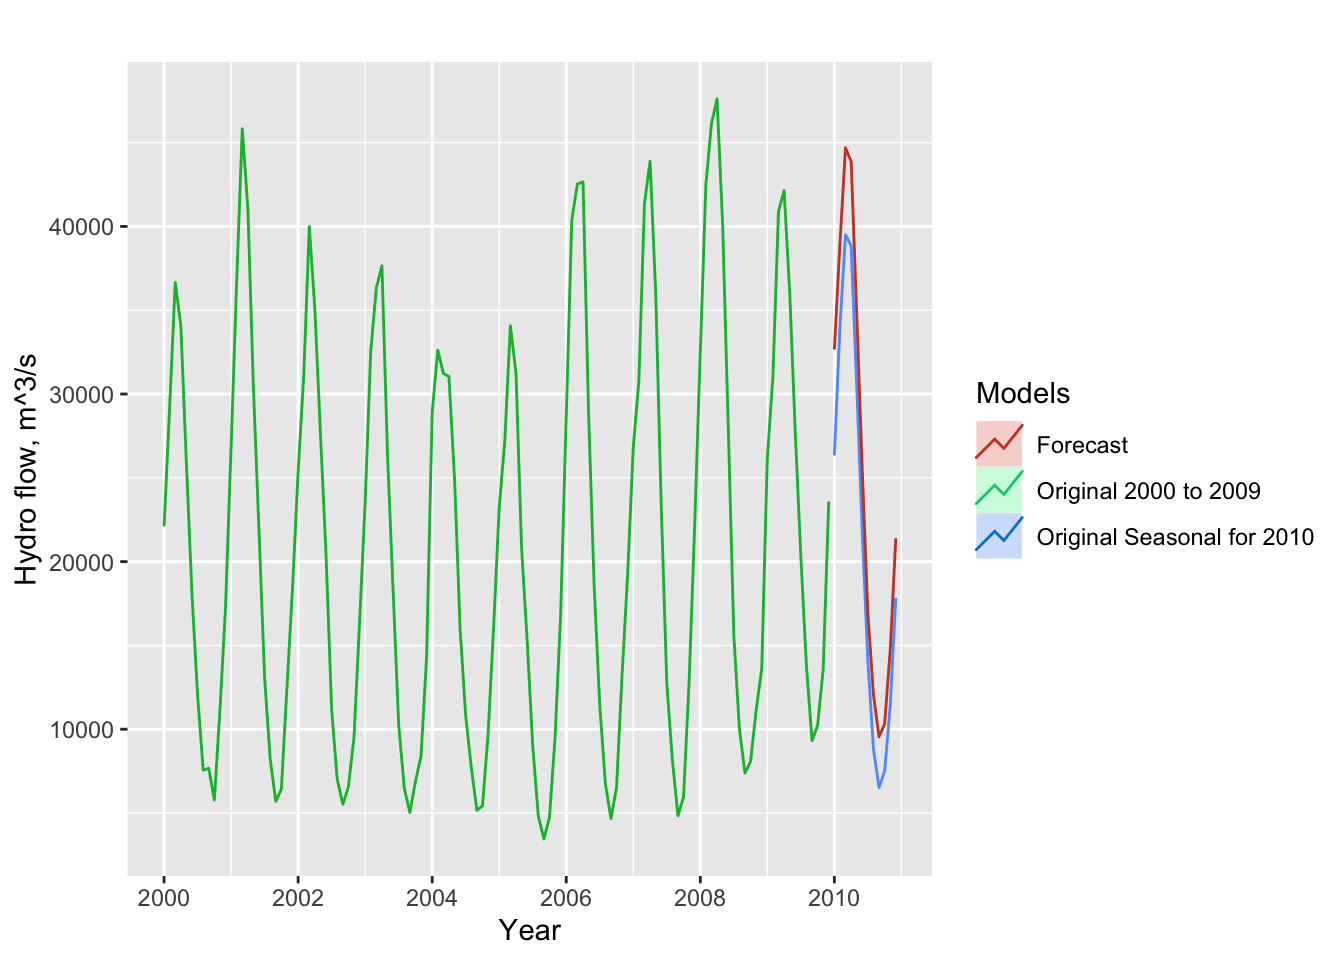
\includegraphics{QiuyingLiao_TSA_A7_Mar20_files/figure-latex/unnamed-chunk-13-1.pdf}

\begin{Shaded}
\begin{Highlighting}[]
\CommentTok{\#Comparing PACFs}
\FunctionTok{par}\NormalTok{(}\AttributeTok{mfrow=}\FunctionTok{c}\NormalTok{(}\DecValTok{1}\NormalTok{,}\DecValTok{4}\NormalTok{))}
\FunctionTok{Pacf}\NormalTok{(ts\_energy\_df\_NG,}\AttributeTok{lag.max=}\DecValTok{40}\NormalTok{,}\AttributeTok{main=}\StringTok{"Natural Gas"}\NormalTok{,}\AttributeTok{ylim=}\FunctionTok{c}\NormalTok{(}\SpecialCharTok{{-}}\DecValTok{1}\NormalTok{,}\DecValTok{1}\NormalTok{))}
\FunctionTok{Pacf}\NormalTok{(NG\_seas\_diff ,}\AttributeTok{lag.max=}\DecValTok{60}\NormalTok{,}\AttributeTok{main=}\StringTok{"Seasonal{-}Differenced Natural Gas"}\NormalTok{,}\AttributeTok{ylim=}\FunctionTok{c}\NormalTok{(}\SpecialCharTok{{-}}\DecValTok{1}\NormalTok{,}\DecValTok{1}\NormalTok{)) }\CommentTok{\#at lag 12}
\FunctionTok{Pacf}\NormalTok{(NG\_trend\_diff,}\AttributeTok{lag.max=}\DecValTok{60}\NormalTok{,}\AttributeTok{main=}\StringTok{"Trend{-}Differenced Natural Gas"}\NormalTok{,}\AttributeTok{ylim=}\FunctionTok{c}\NormalTok{(}\SpecialCharTok{{-}}\DecValTok{1}\NormalTok{,}\DecValTok{1}\NormalTok{)) }\CommentTok{\#at lag 1}
\FunctionTok{Pacf}\NormalTok{(NG\_both\_diff,}\AttributeTok{lag.max=}\DecValTok{60}\NormalTok{,}\AttributeTok{main=}\StringTok{"Twice{-}Differenced Natural Gas"}\NormalTok{,}\AttributeTok{ylim=}\FunctionTok{c}\NormalTok{(}\SpecialCharTok{{-}}\DecValTok{1}\NormalTok{,}\DecValTok{1}\NormalTok{))}
\end{Highlighting}
\end{Shaded}

\includegraphics{QiuyingLiao_TSA_A7_Mar20_files/figure-latex/unnamed-chunk-13-2.pdf}

\begin{Shaded}
\begin{Highlighting}[]
\CommentTok{\#Plot ACF and PACF for twice{-}differenced series {-} Steps 3 (order of non{-}seasonal) and 5 ) order of seasonal}
\FunctionTok{par}\NormalTok{(}\AttributeTok{mfrow=}\FunctionTok{c}\NormalTok{(}\DecValTok{1}\NormalTok{,}\DecValTok{2}\NormalTok{))}
\FunctionTok{Acf}\NormalTok{(NG\_both\_diff,}\AttributeTok{lag.max=}\DecValTok{60}\NormalTok{,}\AttributeTok{main=}\StringTok{"Twice{-}Differenced Natural Gas"}\NormalTok{,}\AttributeTok{ylim=}\FunctionTok{c}\NormalTok{(}\SpecialCharTok{{-}}\DecValTok{1}\NormalTok{,}\DecValTok{1}\NormalTok{))}
\FunctionTok{Pacf}\NormalTok{(NG\_both\_diff,}\AttributeTok{lag.max=}\DecValTok{60}\NormalTok{,}\AttributeTok{main=}\StringTok{"Twice{-}Differenced Natural Gas"}\NormalTok{,}\AttributeTok{ylim=}\FunctionTok{c}\NormalTok{(}\SpecialCharTok{{-}}\DecValTok{1}\NormalTok{,}\DecValTok{1}\NormalTok{))}
\end{Highlighting}
\end{Shaded}

\includegraphics{QiuyingLiao_TSA_A7_Mar20_files/figure-latex/unnamed-chunk-13-3.pdf}

\begin{quote}
Answer: We look at the twice differenced series to identify model order.
We look at the first 12 lags for ACF and PACF we don't see slow decays
but it looks like we have cut offs at lag 2 on both plots indicating on
ARMA (p=2,q=2), and we know from ndiffs that d=1. (p,d,q) = (2,1,2) We
look at the seasonal lags only (12,24,36,48). ACF has one spike at 12
and PACF has 2 spikes one at 12 and one at 24. This is an indication of
a seasonal moving average (SMA). Therefore, the order of seasonal
component is P=0 and Q=1. We know from nsdiffs that D=1. (P,D,Q) =
(0,1,1)
\end{quote}

\hypertarget{q8}{%
\subsubsection{Q8}\label{q8}}

Compare the residual series for Q7 and Q6. Can you tell which ARIMA
model is better representing the Natural Gas Series? Is that a fair
comparison? Explain your response.

\begin{quote}
Answer: I cannot tell which ARIMA moel is better representing the
Natural Gas Series because it it not a fair comparison. They are not
comparable because we are using different models. Q6 is the one that we
only perform on the non-seasoanl component. We assume that seasonal
component is constant and remove that to do this model; for Q7, we put
the seasonal component back to do analysis.
\end{quote}

\begin{Shaded}
\begin{Highlighting}[]
\CommentTok{\#Question 7}
\NormalTok{SARIMA\_manual }\OtherTok{\textless{}{-}} \FunctionTok{Arima}\NormalTok{(ts\_energy\_df\_NG,}\AttributeTok{order=}\FunctionTok{c}\NormalTok{(}\DecValTok{2}\NormalTok{,}\DecValTok{1}\NormalTok{,}\DecValTok{2}\NormalTok{),}\AttributeTok{seasonal=}\FunctionTok{c}\NormalTok{(}\DecValTok{0}\NormalTok{,}\DecValTok{1}\NormalTok{,}\DecValTok{1}\NormalTok{),}\AttributeTok{include.drift=}\ConstantTok{FALSE}\NormalTok{) }
\FunctionTok{print}\NormalTok{(SARIMA\_manual)}
\end{Highlighting}
\end{Shaded}

\begin{verbatim}
## Series: ts_energy_df_NG 
## ARIMA(2,1,2)(0,1,1)[12] 
## 
## Coefficients:
##           ar1     ar2      ma1      ma2     sma1
##       -0.2171  0.7061  -0.0481  -0.9164  -0.7166
## s.e.   0.0826  0.0643   0.0758   0.0729   0.0563
## 
## sigma^2 = 28014069:  log likelihood = -2271.66
## AIC=4555.33   AICc=4555.71   BIC=4575.88
\end{verbatim}

\begin{Shaded}
\begin{Highlighting}[]
\CommentTok{\#Check residuals series}
\FunctionTok{par}\NormalTok{(}\AttributeTok{mfrow=}\FunctionTok{c}\NormalTok{(}\DecValTok{1}\NormalTok{,}\DecValTok{3}\NormalTok{))}
\FunctionTok{ts.plot}\NormalTok{(SARIMA\_manual}\SpecialCharTok{$}\NormalTok{residuals)}
\FunctionTok{Acf}\NormalTok{(SARIMA\_manual}\SpecialCharTok{$}\NormalTok{residuals,}\AttributeTok{lag.max=}\DecValTok{40}\NormalTok{)}
\FunctionTok{Pacf}\NormalTok{(SARIMA\_manual}\SpecialCharTok{$}\NormalTok{residuals,}\AttributeTok{lag.max=}\DecValTok{40}\NormalTok{)}
\end{Highlighting}
\end{Shaded}

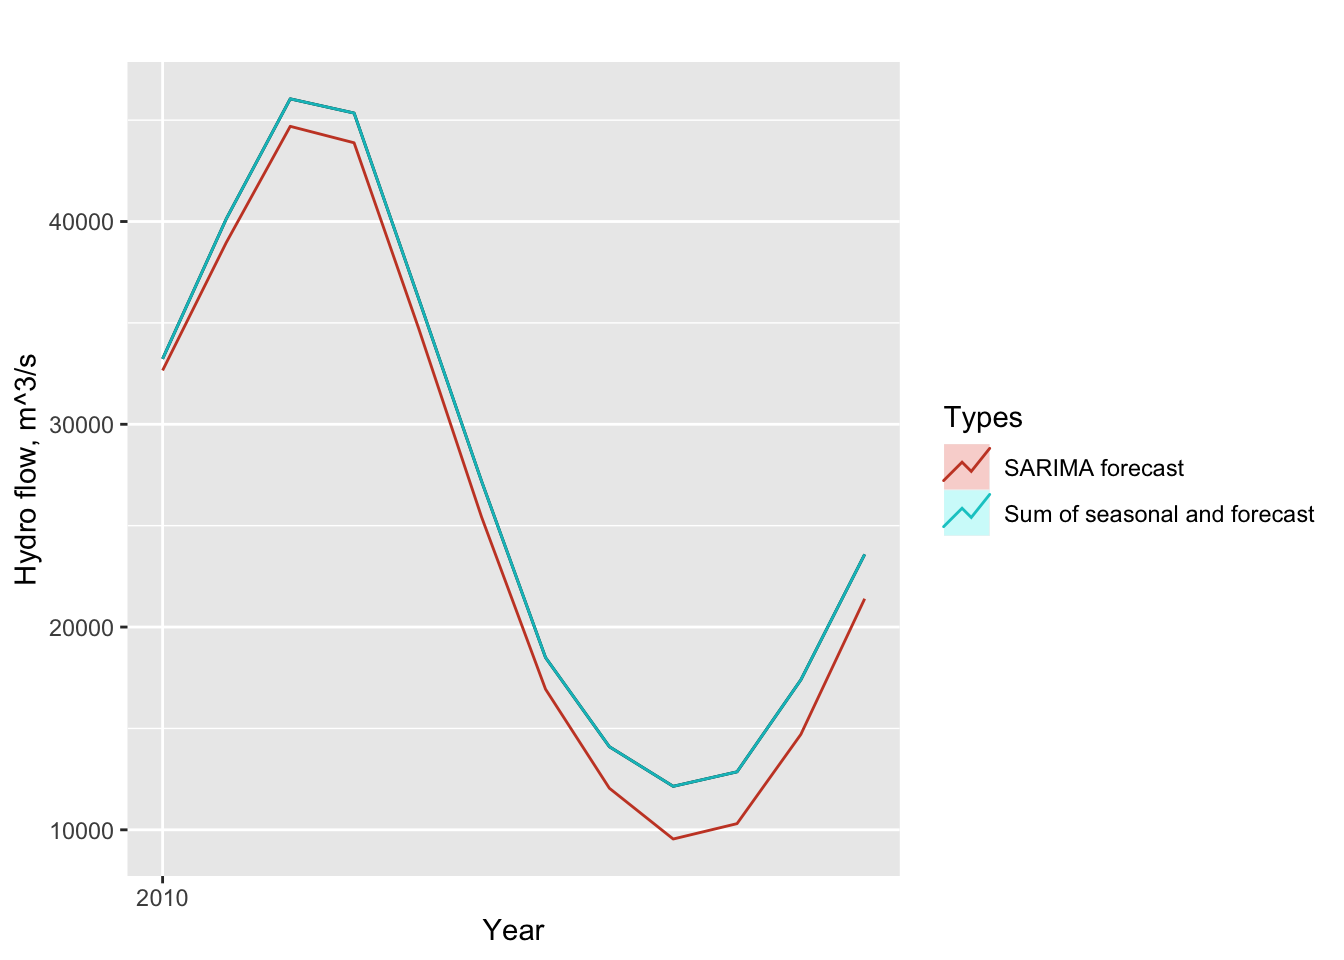
\includegraphics{QiuyingLiao_TSA_A7_Mar20_files/figure-latex/unnamed-chunk-14-1.pdf}

\hypertarget{checking-your-model-with-the-auto.arima}{%
\subsection{Checking your model with the
auto.arima()}\label{checking-your-model-with-the-auto.arima}}

\textbf{Please} do not change your answers for Q4 and Q7 after you ran
the \(auto.arima()\). It is \textbf{ok} if you didn't get all orders
correctly. You will not loose points for not having the same order as
the \(auto.arima()\).

\hypertarget{q9}{%
\subsubsection{Q9}\label{q9}}

Use the \(auto.arima()\) command on the \textbf{deseasonalized series}
to let R choose the model parameter for you. What's the order of the
best ARIMA model? Does it match what you specified in Q4?

\begin{quote}
Answer: the order of the best ARIMA model is (2,1,3). It doesn't match
the ``q'' I specified in Q4 which is q=2.
\end{quote}

\begin{Shaded}
\begin{Highlighting}[]
\NormalTok{ARIMA\_autofit }\OtherTok{\textless{}{-}} \FunctionTok{auto.arima}\NormalTok{(deseasonal\_NG,}\AttributeTok{max.D=}\DecValTok{0}\NormalTok{,}\AttributeTok{max.P =} \DecValTok{0}\NormalTok{,}\AttributeTok{max.Q=}\DecValTok{0}\NormalTok{)}
\FunctionTok{print}\NormalTok{(ARIMA\_autofit)}
\end{Highlighting}
\end{Shaded}

\begin{verbatim}
## Series: deseasonal_NG 
## ARIMA(2,1,3) with drift 
## 
## Coefficients:
##           ar1     ar2     ma1      ma2      ma3      drift
##       -0.3019  0.6482  0.0546  -0.9126  -0.0860  -359.8849
## s.e.   0.0963  0.0930  0.1209   0.0495   0.0999    33.5706
## 
## sigma^2 = 26790433:  log likelihood = -2380.74
## AIC=4775.49   AICc=4775.97   BIC=4799.82
\end{verbatim}

\begin{Shaded}
\begin{Highlighting}[]
\FunctionTok{par}\NormalTok{(}\AttributeTok{mfrow=}\FunctionTok{c}\NormalTok{(}\DecValTok{1}\NormalTok{,}\DecValTok{3}\NormalTok{))}
\FunctionTok{ts.plot}\NormalTok{(ARIMA\_autofit}\SpecialCharTok{$}\NormalTok{residuals)}
\FunctionTok{Acf}\NormalTok{(ARIMA\_autofit}\SpecialCharTok{$}\NormalTok{residuals,}\AttributeTok{lag.max=}\DecValTok{40}\NormalTok{)}
\FunctionTok{Pacf}\NormalTok{(ARIMA\_autofit}\SpecialCharTok{$}\NormalTok{residuals,}\AttributeTok{lag.max=}\DecValTok{40}\NormalTok{)}
\end{Highlighting}
\end{Shaded}

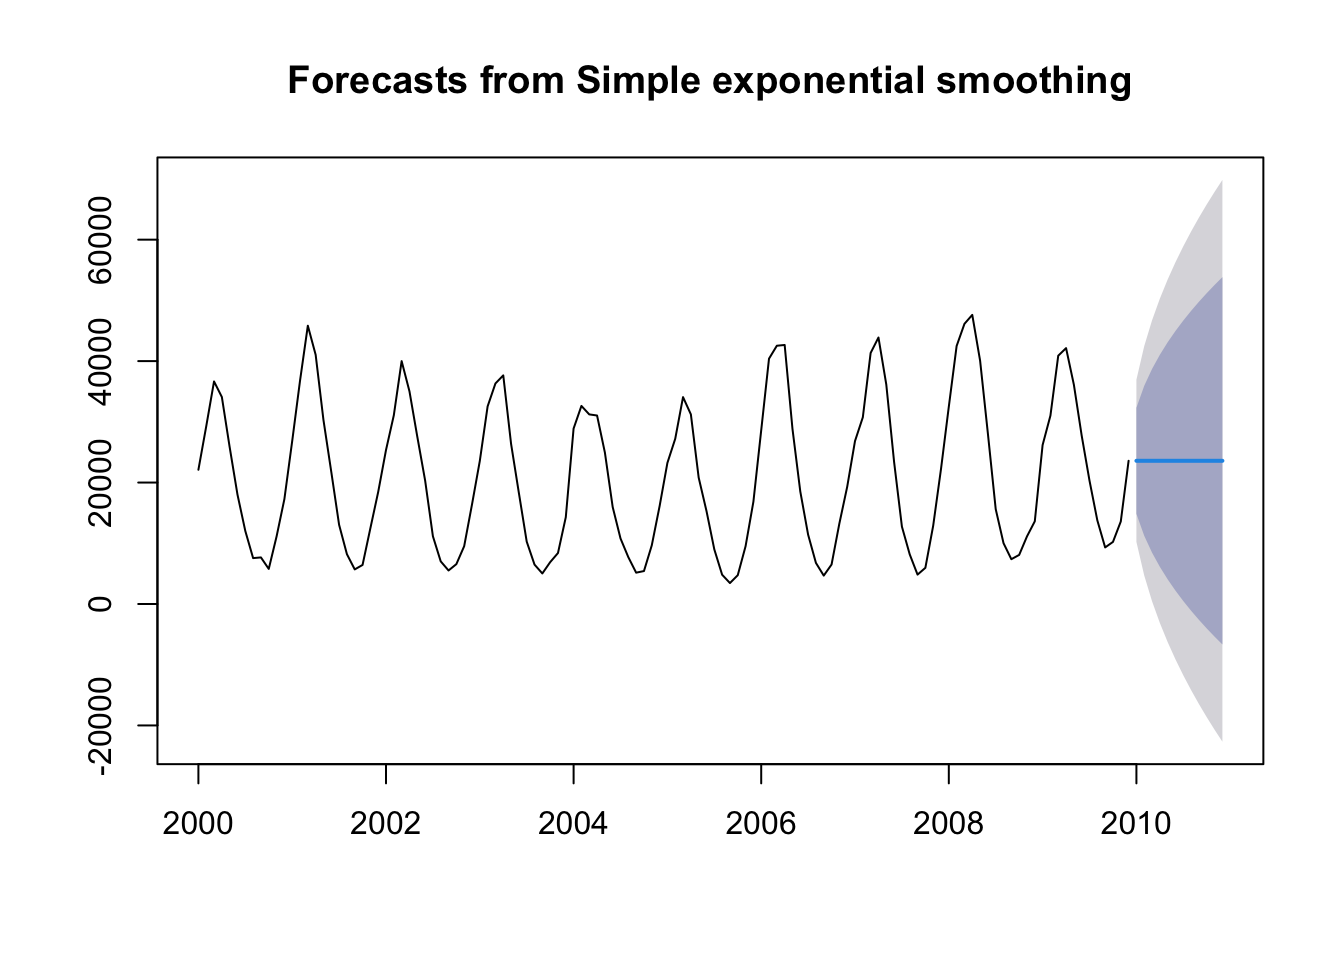
\includegraphics{QiuyingLiao_TSA_A7_Mar20_files/figure-latex/unnamed-chunk-15-1.pdf}

\hypertarget{q10}{%
\subsubsection{Q10}\label{q10}}

Use the \(auto.arima()\) command on the \textbf{original series} to let
R choose the model parameters for you. Does it match what you specified
in Q7?

\begin{quote}
Answer: It doesn't match what I specified in Q7. I specified (2,1,2)
(0,1,1), but R's selection is (2,0,1)(2,1,2)
\end{quote}

\begin{Shaded}
\begin{Highlighting}[]
\NormalTok{SARIMA\_autofit }\OtherTok{\textless{}{-}} \FunctionTok{auto.arima}\NormalTok{(ts\_energy\_df\_NG)}
\FunctionTok{print}\NormalTok{(SARIMA\_autofit)}
\end{Highlighting}
\end{Shaded}

\begin{verbatim}
## Series: ts_energy_df_NG 
## ARIMA(2,0,1)(2,1,2)[12] with drift 
## 
## Coefficients:
##          ar1      ar2      ma1     sar1     sar2     sma1    sma2      drift
##       1.1650  -0.2834  -0.4837  -0.0667  -0.0785  -0.6371  0.0072  -357.8436
## s.e.  0.4164   0.3180   0.3993   1.3208   0.1014   1.3201  0.9205    44.1284
## 
## sigma^2 = 27958166:  log likelihood = -2278.46
## AIC=4574.91   AICc=4575.74   BIC=4605.77
\end{verbatim}

\begin{Shaded}
\begin{Highlighting}[]
\FunctionTok{par}\NormalTok{(}\AttributeTok{mfrow=}\FunctionTok{c}\NormalTok{(}\DecValTok{1}\NormalTok{,}\DecValTok{3}\NormalTok{))}
\FunctionTok{ts.plot}\NormalTok{(SARIMA\_autofit}\SpecialCharTok{$}\NormalTok{residuals)}
\FunctionTok{Acf}\NormalTok{(SARIMA\_autofit}\SpecialCharTok{$}\NormalTok{residuals,}\AttributeTok{lag.max=}\DecValTok{40}\NormalTok{)}
\FunctionTok{Pacf}\NormalTok{(SARIMA\_autofit}\SpecialCharTok{$}\NormalTok{residuals,}\AttributeTok{lag.max=}\DecValTok{40}\NormalTok{)}
\end{Highlighting}
\end{Shaded}

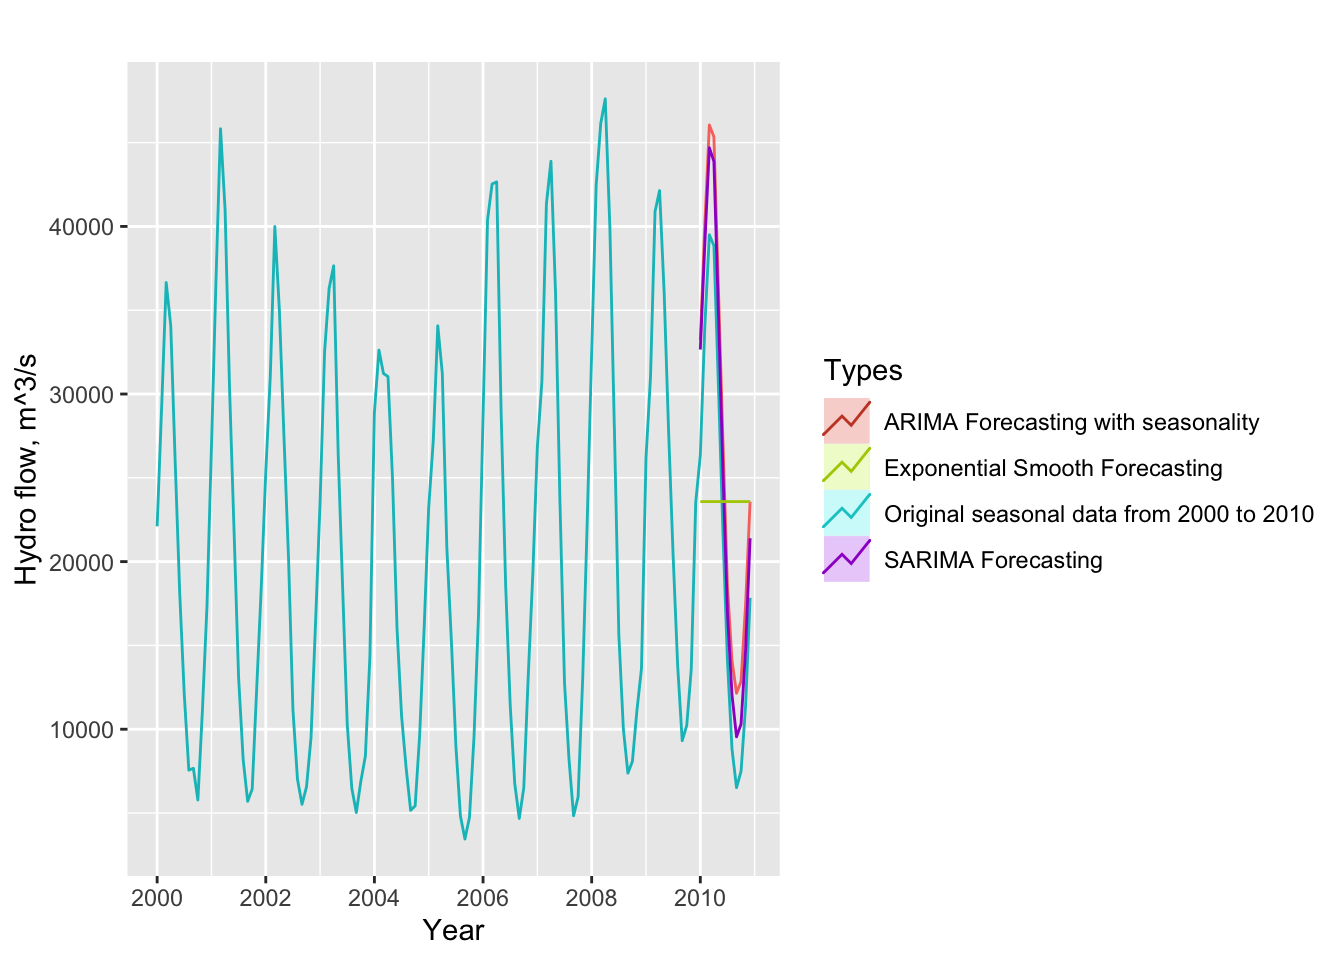
\includegraphics{QiuyingLiao_TSA_A7_Mar20_files/figure-latex/unnamed-chunk-16-1.pdf}

\end{document}
